\chapter{Numbers}
The goal of this textbook is to teach students how to design digital systems.
To understand what this means, it is necessary to understand the behavior of
a digital system.  A digital system is a device which receives binary
numbers as input and generates binary numbers as output.  A binary number
is a number composed of bits, or binary digits.  A bit is equal to 
0 or 1.  Generally, bits are represented by voltages, a 0 by a ground 
potential and a 1 by a 3.3v or 5v potential.  However, for most of this 
text, the physical representation of bits will take a back seat to the
the logical representation.  Figure~\ref{fig:sys} shows 
a digital system with three bits of input and two bits of output.

\begin{figure}[ht]
\center{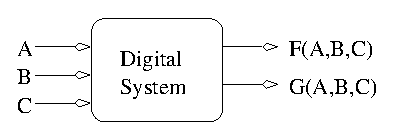
\includegraphics{./Fig1/sys}}
\caption{An abstract digital system with three bits of input
labeled A,B,C and two bits of output, F(A,B,C) and G(A,B,C).}
\label{fig:sys}
\end{figure}

The letters $A,B,C$ in Figure~\ref{fig:sys} represent {\it Boolean variables}, 
\index{Boolean variable} variables which are only allowed to assume the values 
0 or 1.  The notation $F(A,B,C)$ means that the output depends on the values 
of $A,B,C$. 

Unfortunately, there is a disconnect between the normal way of describing
quantities using the digits $0 \ldots 9$ and that used by digital systems
using the bits $0,1$.  The study of digital systems starts by describing
the numbering system used to describe decimal numbers and binary numbers.  
These systems are
{\it positional numbering systems} \index{numbering system!positional} 
- the position of a digit in a number determines its significance.  The
familiar decimal numbering system is used to illustrate the main concepts
in positional numbering system.

\section{Decimal}
The goal of any numbering system (this includes both
decimal and binary) is to represent quantities using a fixed set of
symbols.  One feature which distinguishes numbering systems is 
the number of symbols used to represent quantities, the numbering 
system's {\it base} \index{numbering system!base}.

Decimal is a base-10 numbering system where quantities are expressed using 
10 symbols $\{0,1,2,3,4,5,6,7,8,9\}$.  To explicitly denote a 
number's base, include the base as a subscript after the number.  For example, 
the number of days in a year could be represented as $365_{10}$. 

Each digit in a number represents a quantity which depends on the digit, 
the base, and the position of the digit.  The value of a digit is determined 
by the formula $d * b^i$ where $d$ is the digit, $i$ is the position of the 
digit and $b$ is the base.  The position of the digit immediately to the 
left of the decimal point is 0, every other digit is indexed starting from 
this position.  The value of a multidigit number is the sum of the values of 
the digits, $\sum_{i=0}^N d_i*b^i$, where $N$ is the number of digits in
the number.  Thus $365_{10}$ is interpreted as 
$$3*10^2 + 6*10^1 + 5*10^0 $$

The leftmost digit is called the most significant
digit and the rightmost digit is called the least 
significant digit.  

\section{Binary}
Binary is a base-2 numbering system where quantities are expressed using
two symbols $\{0,1\}$.  When verbally communicating a binary value like $101_2$,
do not say ``one hundred and one base two".  The term {\it hundred} is a decimal 
concept and implies the quantity being described is decimal, contradicting
the ``base two".  Instead,  say ``one zero one base two", with the ``base
two" part being optional.   Enough about the nomenclature used to communicate
binary numbers, how to represent values in binary?  Since binary is a 
positional numbering system, then apply the formula $\sum_{i=0}^N d_i*b^i$.

\subsection{Binary to Decimal}
The value of $101_2$ is interpreted as 
$$101_2 = 1*2^2 + 0*2^1 + 1*2^0 = \\
1*4_{10} + 0*2_{10} + 1*1_{10} = \\
4_{10} + 0_{10} + 1_{10} = 5_{10}$$

Application of the positional numbering formula to a binary number
converts it into a decimal number.  As in the decimal case 
there are special names for two of the bits. The leftmost bit is 
called the most significant bit (MSB) and the 
rightmost bit is called the least significant 
bit (LSB).  As a final example, convert $1101_2$ to decimal.

$$1*2^3 + 1*2^2 + 0*2^1 + 1*2^0 = \\
1*8_{10} + 1*4_{10} + 0*2_{10} + 1*1_{10} = \\
8_{10} + 4_{10} + 0_{10} + 1_{10} = 13_{10}$$
\label{page:bin2dec}


\subsection{Decimal to Binary}
In order to provide inputs to a digital system, real world values
represented in decimal need to be converted into binary.
While there are several ways to perform
this conversion, it makes sense to adapt a familiar procedure, 
the binary to decimal conversion.  The key idea is to represent the 
decimal number as the sum of distinct powers-of-two.  To assist in this
procedure, use a power-of-two table.
\\ \\
\begin{tabular}{|c|c|c|c|c|c|c|c|c|c|c|}\hline
$i$   & 0 & 1 &  2 &  3 &  4 &  5 &  6 &  7  &  8  &  9  \\ \hline
$2^i$ & 1 & 2 &  4 &  8 & 16 & 32 & 64 & 128 & 256 &  512\\ \hline 
\end{tabular}
\\ \\
The power-of-two table lists indices, $i$, and its value when it is
raised to the exponent of 2.  This table is used in the following
3-step decimal to binary conversion procedure.

\begin{description}
\item [Step 1] Find the largest power of two less than or equal to the 
number to convert.  
\item [Step 2] Subtract this power of two from the number being converting.
This is the remaining number to convert.
\item [Step 3] If the reminder is not equal to 0, go to step 1; otherwise stop.
\end{description}

The set of values found in Step 1 are the distinct powers-of-two that
when added together equal the number to be converted.  The conversion
is completed by putting the sum into the positional numbering notation.  
The procedure is now applied to convert $13_{10}$ into binary.

\begin{tabular}{ll}
Step & Action \\
1 & The largest power-of-two less than or equal to 13 is 8. \\
2 & The remaining number to convert is 13-8=5. \\
3 & The new remainder is not 0. \\
1 & The largest power-of-two less than or equal to 5 is 4. \\
2 & The remaining number to convert is 5-4=1. \\
3 & The new remainder is not 0. \\
1 & The largest power-of-two less than or equal to 1 is 1. \\
2 & The remaining number to convert is 1-1=0. \\
3 & The new remainder is 0 so the conversion is complete. \\
\end{tabular}

Thus, $13_{10} = 8+4+1$.  This derivation can also be expressed in the
positional numbering notation as follows.

$$13_{10} = 8_{10} + 4_{10} + 1_{10} = 1*2^3 + 1*2^2 + 1*2^0 $$

At this point the ``missing" powers of two are included in the
summation by setting their coefficients to 0.  In the final step, all
the coefficients are stripped off to form the binary number.  Continuing
with the previous example,

$$13_{10} = 1*2^3 + 1*2^2 + 0*2^1 + 1*2^0 = 1101_2$$

Notice that this derivation is the exact reverse of the binary to
decimal conversion shown on page~\pageref{page:bin2dec}.  


\label{page:two-to-N}
What range of values can be described by $N$ bits?  Clearly, the smallest 
number to be represented is 0.  To determine the largest number 
calculate how many different binary numbers can be formed with $N$ bits.
Each bit can be written in two different ways, 0 or 1. Since these choices
are independent events, then the total number of 
possible outcomes is the product of the individual events.  Hence, the 
number of ways to arrange $N$ bits is equal to $2*2* \ldots *2$ ($N$ times) 
which is equal to $2^N$.  Thus, $N$ bits can be arranged in $2^N$ different 
ways. Since 0 is the smallest binary number then the maximum binary number
is $2^N-1$.  The range of an $N$-bit binary number can be represented
as $[0,2^{N}-1]$, where the $[$ and $]$ symbols mean that values 0 and
$2^{N}-1$ are included in the range. 


\section{Hexadecimal}
Hexadecimal is a base-16 numbering system where quantities are expressed using
16 symbols $\{0,1,2,3,4,5,6,7,8,9,A,B,C,D,E,F\}$.  The symbols
$\{A \ldots F \}$ represent quantities just like the symbols $\{0 \ldots 9 \}$.
The symbol $A$ represents the quantity 10, $B$ 11, $C$ 12, $D$ 13, $E$ 14, and
$F$ 15.  So if humans had adopted the hexadecimal numbering system instead of 
decimal you might say to a friend, ``I had $A$ friends over for a party last 
night"  meaning that 10 people showed up. To show how hexadecimal is used 
as a shorthand for binary, consider the conversion of hexadecimal numbers
into binary.

\subsection{Hexadecimal to Binary}
To convert a number from hexadecimal to binary, {\it unpack} it.  That is, 
each hexadecimal digit is converted into a 4-bit binary representation.  
This conversion 
is possible because four bits exactly represents every hexadecimal digit
as shown in Table~\ref{table:First16}.

\begin{table}
\begin{center}
\begin{tabular}{|c|c|c|c|}\hline
Decimal & Binary & Hexadecimal \\ \hline
0	& 0000	& 0	 \\ \hline
1	& 0001	& 1	 \\ \hline
2	& 0010	& 2	 \\ \hline
3	& 0011	& 3	 \\ \hline
4	& 0100	& 4	 \\ \hline
5	& 0101	& 5	 \\ \hline
6	& 0110	& 6	 \\ \hline
7	& 0111	& 7	 \\ \hline
8	& 1000	& 8	 \\ \hline
9	& 1001	& 9	 \\ \hline
10	& 1010	& A	 \\ \hline
11	& 1011	& B	 \\ \hline
12	& 1100	& C	 \\ \hline
13	& 1101	& D	 \\ \hline
14	& 1110	& E	 \\ \hline
15	& 1111	& F	 \\ \hline
\end{tabular}
\caption{The first 16 counting numbers represented in 
decimal, binary, and hexadecimal.}
\label{table:First16}
\end{center}
\end{table}

In order to convert $1DAD_{16}$ to binary, replace each hexadecimal
digit with its binary counterpart by consulting Table~\ref{table:First16}.
For example $1DAD_{16} = 0001~1101~1010~1101_{2}$.  The spaces between the
binary numbers are included to make reading the number easier.

\subsection{Binary to Hexadecimal}
The above procedure can be reversed to convert binary numbers into 
hexadecimal.  Group the bits into sets of four, starting at the least
significant bit, then convert each set of four bits into its corresponding
hexadecimal digit in Table~\ref{table:First16}.  
If there are not four digits in the most significant 
grouping, then just add 0s to make a grouping of three -- that is 
pad the number with zeros.  For example, convert  $1110101011_2$ into 
hexadecimal. $1110101011_2 = 0011~1010~1011 = 3AB_{16}$.

To understand why this conversion works, consider the binary 
number $1110101011_2$.  Start by writing down this number using the 
technique from the previous section and then convert it to hexadecimal.
\\ \\
{\tiny
$\begin{array}{l}
1110101011_2= \\
1*2^9+1*2^8+1*2^7+0*2^6+1*2^5+0*2^4+1*2^3+0*2^2+1*2^1+1*2^0 = \\
2^8(0*2^3+0*2^2+1*2^1+1*2^0) + 2^4(1*2^3+0*2^2+1*2^1+0*2^0) + 2^0*(1*2^3+0*2^2+1*2^1+1*2^0) =\\
2^8(0011_2) + 2^4(1010_2) +  2^0(1011_2) =\\
2^{4*2}(0011_2) + 2^{4*1}(1010_2) +  2^{4*0}(1011_2) =\\
16^2(0011_2) + 16^1(1010_2) + 16^0*(1011_2) =\\
16^2(3_{16}) + 16^1(A_{16}) + 16^0*(B_{16}) =\\
3AB_{16}
\end{array}$
} 


\section{Addition of Binary Numbers}
\label{page:addition}
The fact that the addition of binary numbers is similar to the 
addition of decimal numbers should not come as a surprise as both
are positional numbering systems. However, when adding binary numbers
with a digital system, it is possible that the result may exceed the
digital system's capacity because the digital system can only accommodate a 
finite number of bit positions.  The number of bits to be 
simultaneously manipulated by a digital system is refereed to as 
its {\it word size} \index{word size}.  A digital system with a
word size of N-bits can represent binary numbers in the range 
$[0, 2^N-1]$.  {\it Overflow} \index{overflow} occurs when a 
digital system is forced to represent a value outside the range 
of its word size.

The process of adding binary numbers is exactly the same as adding
decimal numbers: Start in the LSB and work towards the 
MSB.  Each of the bit-positions is called a {\it bit-slice} 
\index{bit-slice}.  At each bit-slice, the two bits of the sum are
added together along with the carry-in generated in the previous 
bit-slice.  This addition in a bit-slice will generate one bit of 
sum and possibly one bit of carry to the next bit-slice. The addition 
of bits must be performed in base-2, hence the results may look 
strange.  For example, $1_2 + 1_2 = 10_2$. In this case the sum-bit 
equals 0 and the carry-bit equals 1.  Now, consider a more 
complex problem, adding $3+2$ in binary, assuming a word size of 
four bits.  
\\ \\
\begin{tabular}{r|rrrr}
    &   & 1 &   &    \\
 3  & 0 & 0 & 1 & 1  \\
+2  & 0 & 0 & 1 & 0  \\ \hline
 5  & 0 & 1 & 0 & 1  \\ 
\end{tabular}
\\ \\
Notice, one of the additions produced a carry which is
propagated to the next significant bit position.
The next example demonstrates an addition where the 
result is larger than the word size can accommodate.
\\ \\
\begin{tabular}{r|rrrrr}
    & 1 & 1 & 1 & 1 & 1  \\
13  &   & 1 & 1 & 0 & 1  \\ 
+7  &   & 0 & 1 & 1 & 1  \\ \hline
20  & 1 & 0 & 1 & 0 & 0  \\
\end{tabular}
\\ \\
The decimal result, 20, cannot be represented in four bits, hence
the addition produced overflow.  When adding binary numbers,
overflow occurs whenever there is a carry-out from the most
significant bit-slice.  That is, the result requires more bits 
than are available in the word size.

After being introduced to binary numbering it might be tempting
to look at all collections of bits as being binary numbers.
In truth, a collection of bits has no implicit meaning.  The 
sequence of bits, 0101, could just as easily represent the 
value 5 as it could represent the intensity of red on a display.
A collection of bits gets its meaning from the interpretation
used.  When bits are used to represent integer quantities, 
two main interpretations, binary numbering and 2's complement,
predominate.
 
\section{Negative Numbers}
The binary numbering systems is often called an {\it unsigned}
numbering representation.  The term unsigned arises from the 
fact that there is no need to write a sign symbol in front of
a binary number because all binary numbers are positive --
the positive sign is implicit.  A {\it signed} numbering representation, 
2's complement, is capable of representing both positive and 
negative numbers.

Like binary numbering, 2's-complement numbers exist within the 
confines of a word size.  One way to determine the 2's-complement 
representation of a decimal number $x$, is to write 
down the binary representation for the quantity $2^N+x$ using 
$N$ bits, where $N$ is the word size.  For example, assuming a 
word size of four bits, determine the 2's-complement representation 
for 6.  To do this, compute $2^N + x = 2^4 + 6 = 16+6=22 = 10110_2$.  
Taking the least significant four bits yields $0110$.  

There are two
points to note.  First, this representation is the same as in 
binary numbering.  Second, the 2's-complement value is written
without a subscript 2, because it is not a binary number.  Now
consider the 2's-complement representation of a negative number.

Assuming a word size of four bits, determine the 2's-complement
representation for -6.  Compute 
$2^N + x = 2^4 - 6 = 16-6 = 10 = 01010_2$.  Taking the least
significant four bits yields $1010$.  

To determine the decimal value of a 2's-complement number,
inspect its MSB.  If the MSB is 0, then the number is
positive, hence can be interpreted as a binary number.
If the MSB is 1, then $2^N+x$ must be solved for $x$.
There is, however an easier way to approach this problem.

Negating a 2's-complement number will mean changing 
the sign of the underlying decimal representation.  The
negation of a 2's-complement number, $x$, can be formed
by flipping all the bits of $x$ and then adding 1.  For
example, take the complement of the 4-bit 2's-complement 
number $x=0110$ which equals 6.  Flipping all 
the bits of $x$ yields $1001$.  Adding 1 to this yields 
$1010$, which was previously shown to equal -6. 

This technique aids in interpreting negative 2's-complement 
numbers as follows.  Given a 2's-complement number that is 
negative, form its
negation, convert that to decimal, then stick a negative
sign in front of the decimal representation.  For example,
determine the decimal representation for the 4-bit 2's-complement 
quantity 1010.  Since the MSB is 1, this
2's-complement number represents a negative quantity.
Flipping the bits, 0101, then adding 1, results in 0110.  
This is the representation for 6, so the original 2's-complement 
number 1010 represent -6.

Figure~\ref{fig:2wheel} shows every combination of four bits
and their associated 2's-complement representation.

\begin{figure}[ht]
\center{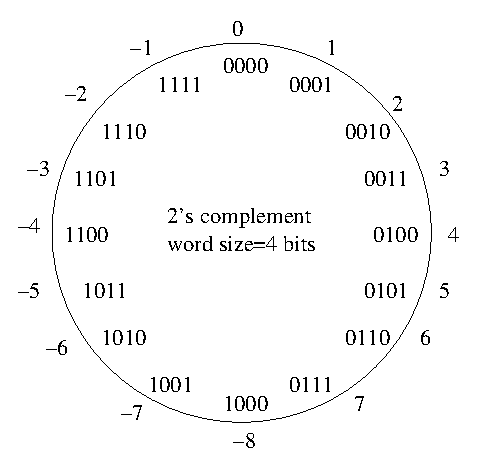
\includegraphics{./Fig1/2wheel}}
\caption{All possible combinations of four bits and their 2's-complement
interpretations.}
\label{fig:2wheel}
\end{figure}

Clearly, half of the numbers in Figure~\ref{fig:2wheel} have
a leading 0 as their MSB, and are positive; 0 is considered 
a positive number.  The other half of the numbers have their
MSB equal to 1 and are negative.  Since 0 is considered a 
positive number, the largest negative number is 1 larger 
than the largest positive number.  Given a word size of $N$ 
bits the range of 2's-complement numbers is $[-2^{N-1}, 2^{N-1}-1]$.

2's-complement numbers are added in the same way that
binary numbers are added as shown in the 
following three problems.

{\small
\begin{tabular}{ccc}
\begin{tabular}{r|rrrrr}
     &   &   &   &   &     \\
   6 &   & 0 & 1 & 1 & 0   \\
+ -7 &   & 1 & 0 & 0 & 1   \\ \hline
= -1 &   & 1 & 1 & 1 & 1   \\
\end{tabular}
&
\begin{tabular}{r|rrrrr}
     & 1 & 1 & 1 &   &     \\
   3 &   & 0 & 0 & 1 & 1   \\
+ -2 &   & 1 & 1 & 1 & 0   \\ \hline
=  1 &   & 0 & 0 & 0 & 1   \\
\end{tabular}
&
\begin{tabular}{r|rrrrr}
     &   & 1 & 1 &   &     \\
   6 &   & 0 & 1 & 1 & 0   \\
+  6 &   & 0 & 1 & 1 & 0   \\ \hline
= 12 &   & 1 & 1 & 0 & 0   \\
\end{tabular} \\
\end{tabular}
}

The first example, 
$6 + -7$, shows  the addition process working correctly when
the operands have different signs.  The other two problems 
illustrate the need for a new definition of overflow for 2's-complement 
numbers.  The general rule for overflow in 2's complement 
is, \label{page:Ovf} if the carry-in and carry-out 
into and out from the MSB are not equal, then overflow has 
occurred.  The carry-out from the MSB is always thrown away.
For example, the carry-in and carry-out of the MSB in second
problem are both 1, hence the result is valid.  In the third
problem, the carry in to the MSB is 1 and the carry-out from the
MSB is 0, hence overflow has occurred.  This result should not be a 
surprise because the expected result, 12, cannot be represented
as a 4-bit 2's-complement number.

Taking the complement of a 2's-complement number allows subtraction
problems to be converted into addition problems.  \label{page:2sub}
For example, the subtraction problem $3 - 2$ can be rewritten as 
$3 + (-2)$.

\begin{tabular}{ccc}
\begin{tabular}{r ccccc}
   3 &   & 0 & 0 & 1 & 1   \\
- +2 &   & 0 & 0 & 1 & 0   \\ \hline
\end{tabular} 
& Becomes &
\begin{tabular}{r ccccc}
     & 1 & 1 & 1 &   &     \\
   3 &   & 0 & 0 & 1 & 1   \\
+ -2 &   & 1 & 1 & 1 & 0   \\ \hline
=  1 &   & 0 & 0 & 0 & 1   \\
\end{tabular} \\

\end{tabular}
\\ \\
Situations will arise which require increasing the number of bits 
required to represent a number while retaining the value of the
number.  For example, imagine having a 
4-bit binary number that must be stored in a device that holds 
eight bits.  How can this be done while preserving
the magnitude of the number?  For binary numbers, the answer is
easy, add 4 leading zeros, an operation called {\it padding with 0s}.  

For 2's-complement numbers this 
solution will not work.  For example, consider the
4-bit 2's-complement representation for -1 (1111) that needs to
be store in a 8-bit device.  Adding 4 leading 0s 
will change the value of the number to 00001111, the value 
15.  The solution, in this case, is to pad with 1s, yielding
11111111, which represents -1 in 8-bit 2's complement.  As 
with the binary numbering example,
positive 2's-complement numbers can be padded with 0s and
still retain their value.  The general rule for padding
in 2's complement is called {\it sign extension}; 
\index{sign extension} \label{page:2sPad} and involves copying 
the MSB to fill in the needed space.  
Table~\ref{table:SignExt} shows five examples of sign extension
on 2-bit 2's-complement numbers.

\begin{table}
\begin{center}
\begin{tabular}{l|l}
4-bit 2's complement & 8-bit 2's complement \\ \hline
1110=-2			& 11111110=-2 \\ \hline
1010=-6			& 11111110=-6 \\ \hline
1000=-8			& 11111000=-8 \\ \hline
0011=3			& 00000011=3 \\ \hline
0111=7			& 00000111=7 \\ 
\end{tabular}
\caption{Five examples showing how to sign-extend a 4-bit
2's-complement number.}
\label{table:SignExt}
\end{center}
\end{table}

\section{Other codes}

\subsection{Octal}
\pagebreak
.
\pagebreak
.

\subsection{Grey Code}
\pagebreak
.

\subsection{Ones Hot}

\subsection{ASCII}

\subsection{BCD}
\pagebreak
.

\subsection{Fixed Point}
\pagebreak
.

\subsection{Floating Point}
\pagebreak
.
\pagebreak
.



\section{Exercises}
\section{Exercises}
\label{section:chap01Exercises}

\begin{enumerate}
\item \textbf{ (1 pt. each)} Syllabus:
	\begin{enumerate}
	\item What is the late penalty for homework?
	
	\begin{onlysolution}
	\itshape
	There is a 33\% deduction per day.
	\end{onlysolution}

	\item True or False: Calculators can be used during exams.
	
	\begin{onlysolution}
	\itshape
	You cannot use calculators at my exams.
	\end{onlysolution}
	
	
	\item True of False: University ID is required during exams.
	
	\begin{onlysolution}
	\itshape
	I check ID at the exams.  After I learn 
		your names its not such a big
		deal, but bring it to be safe.
	\end{onlysolution}
	
	\item What is my thesis regarding grades?
	{\begin{onlysolution}
		\fcolorbox{red}{yellow}{lorem ipsum}	
	\end{onlysolution}}	
	\item Bob L. Student has the following grades.  Determine his final
	overall course percentage and grade.

		\begin{tabular}{l|l}
		Component & Percentage \\ \hline \hline
		Homework & $60\%$ \\ \hline
		Exam 1	 & $90\%$ \\ \hline
		Exam 2	 & $80\%$ \\ \hline
		Final	 & $70\%$ \\ 
		\end{tabular}


	\begin{onlysolution}
	\itshape
                \begin{tabular}{l|l|l}
                Component & Percentage & Weight \\ \hline \hline
                Homework & $60\%$    & 60*0.35 = 21\\ \hline
                Exam 1   & $90\%$    & 90*0.20 = 18\\ \hline
                Exam 2   & $80\%$    & 80*0.20 = 16\\ \hline
                Final    & $70\%$    & 70*0.25 = 17.5 \\ \hline
                Total    & $72.5\%$ & C \\
                \end{tabular}
	\end{onlysolution}

	\item How should you prepare for the 43$^{rd}$ lecture?

	\begin{onlysolution}
	\itshape
	 Look over homework problem 8.10, page 165
	 \end{onlysolution}
	 
	\end{enumerate}

\item \textbf{ (1 pt. each)} Convert the following numbers to decimal. 
Show work, or receive 1/2 credit.
	\begin{enumerate}
	\item $100_2$
	\begin{onlysolution}	\itshape $100_2 = 2^2 = 4_{10}$\end{onlysolution}
	
	\item $1000_2$
	\begin{onlysolution}	\itshape $1000_2 = 2^3 = 8_{10}$\end{onlysolution}
	
	\item $10000_2$
	\begin{onlysolution}	\itshape $10000_2 = 2^4 = 16_{10}$\end{onlysolution}
	
	\item $100000_2$
	\begin{onlysolution}	\itshape $100000_2 = 2^5 = 32_{10}$\end{onlysolution}
	
	\item $111111_2$
	\begin{onlysolution}	\itshape $111111_2 = 2^5+2^4+2^3+2^2+2^1+2^0=63_{10}$\end{onlysolution}
	
	\item $1000100101000101_2$
	\begin{onlysolution}	\itshape $1000100101000101_2=2^{15}+2^{11}+2^8+2^6+2^5+2^0=35141_{10}$\end{onlysolution}
	
	\item $3EA_{16}$
	\begin{onlysolution}	\itshape$3EA_{16}=0011 1110 1010 = 2^9+2^8+2^7+2^6+2^5+2^3+2^1=1002_{10}$\\ {\color{blue} $3EA_{16} = 3*16^2 +14*16^1 + 10 * 16^0 = 1002_{10} $}\end{onlysolution}
	
     \end{enumerate}


\item \textbf{ (1 pt. each)} Convert the following number to binary. Show 
work, or receive 1/2 credit.
	\begin{enumerate}
	\item $44_{16}$
	\begin{onlysolution}	\itshape $44_{16} =0100 0100_2$\end{onlysolution}
	
	\item $44_{10}$
	\begin{onlysolution}	\itshape $44_{10} = 32+8 = 2^5+2^3=101100_2$\end{onlysolution}
	
	\item $1023_{10}$
	\begin{onlysolution}	\itshape$1023_{10} = 512+256+128+64+32+16+8+4+2+1=
        2^9+2^8+2^7+2^6+2^5+2^4+2^3+2^2+2^1+2^0=1111111111_2$\end{onlysolution}
        
	\end{enumerate}


\item \textbf{ (1 pt. each)} Convert the following number to hex. Show work, or receive 1/2 credit.
	\begin{enumerate}
	
	\item $101011101_2$
	\begin{onlysolution}	{\color{blue} \itshape$0001\, 0101\, 1101_2 = 15D_{16}$} \end{onlysolution}
	
	\item $77_{10}$
	\begin{onlysolution}	\itshape $77_{10} = 64+8+4+1=2^6+2^3+2^2+2^0=100\, 1101_2=4D_{16}$ \end{onlysolution}
	
	\end{enumerate}


\item \textbf{ (2 pts. each)} Toughies:
	\begin{enumerate}
	\item Convert $123_5$ to base-12
	\begin{onlysolution} 	\itshape
		$123_5 = 1*5^2 + 2*5^1 + 3*5^0 = 25+10+3=38_{10}=
        3*12^1 + 2*12^0 = 32_{12}$ \end{onlysolution}
        
	\item Convert $789_{12}$ to base-5
	\begin{onlysolution}
	\itshape	$789_{12} = 7*12^2+8*12^1+9*12^0=1008+96+9=1113_{10}= \\
        1*5^4+3*5^3 + 4*5^2 + 2*5^1 + 3*5^0 = 13423_5$ \end{onlysolution}
        
	\item What is the largest base-10 quantity that can be represented
	using 5 digits in base 12?

	\begin{onlysolution}
	\itshape $BBBBB_{12} = 11*12^4+11*12^3+11*12^2+11*12^1+11*12^0=248831_{10}$ \end{onlysolution}
	
	\end{enumerate}


\item \textbf{ (1 pt. each)} Perform the following additions, assume a word 
size of four bits. Determine if overflow occurs.
	\begin{enumerate}
	{ \color{blue} % every answer changed, questions caught in the crossfire
	\item $0110_2 + 0101_2$
	\begin{onlysolution}\begin{align*}
	1\0\0\0 &\\
	0110 &\\
 +\:0101 &\\[-2ex]
 \rule{9ex}{1pt}\hspace{-1ex}&\\[-1ex]
	1011& \end{align*}\end{onlysolution}
	
	\item $0010_2 + 0110_2$
	\begin{onlysolution}\begin{align*}
	11\0\0 &\\
    0010 &\\
 +\:0110 &\\[-2ex]
 \rule{9ex}{1pt}\hspace{-1ex}&\\[-1ex]
    1000 &\end{align*}\end{onlysolution}
	
	\item $0111_2 + 0011_2$
	\begin{onlysolution}\begin{align*}
	111\0&\\
    0111&\\
 +\:0011&\\	
 \rule{9ex}{1pt}\hspace{-1ex}&\\[-1ex]
	1010 &\end{align*}\end{onlysolution}
	
	\item $0010_2 + 0101_2$
	\begin{onlysolution}\begin{align*}
	0010&\\
 +\:0101&\\
 \rule{9ex}{1pt}\hspace{-1ex}&\\[-1ex]
    0111 &\end{align*}\end{onlysolution}
	
	\item $0010_2 + 1010_2$
	\begin{onlysolution}	\itshape\begin{align*}
	 1\0\0 &\\
	0010 &\\
 +\:1010 &\\
 \rule{9ex}{1pt}\hspace{-1ex}&\\[-1ex]
    1101 &\end{align*}\end{onlysolution}
	
	\item $0101_2 + 1011_2$
	\begin{onlysolution}\begin{align*}
   1111\0&\\
    0101&\\
 +\:1011&\\
    \hline
    0000&\quad\text{\textit{Overflow}} \end{align*}\end{onlysolution}
	
	\item $0011_2 + 1001_2$
	\begin{onlysolution}	\begin{align*}
     11\0&\\
    0011&\\
 +\:1001&\\
    \hline
    1100&\end{align*}\end{onlysolution} }
	
	\end{enumerate}
\end{enumerate}

